\documentclass{chi2009}
\usepackage{times}
\usepackage{url}
\usepackage{graphics}
\usepackage{color}
\usepackage[pdftex]{hyperref}
\hypersetup{%
pdftitle={Your Title},
pdfauthor={Your Authors},
pdfkeywords={your keywords},
bookmarksnumbered,
pdfstartview={FitH},
colorlinks,
citecolor=black,
filecolor=black,
linkcolor=black,
urlcolor=black,
breaklinks=true,
}
\newcommand{\comment}[1]{}
\definecolor{Orange}{rgb}{1,0.5,0}
\newcommand{\todo}[1]{\textsf{\textbf{\textcolor{Orange}{[[#1]]}}}}

\pagenumbering{arabic}  % Arabic page numbers for submission.  Remove this line to eliminate page numbers for the camera ready copy

\begin{document}
% to make various LaTeX processors do the right thing with page size
\special{papersize=8.5in,11in}
\setlength{\paperheight}{11in}
\setlength{\paperwidth}{8.5in}
\setlength{\pdfpageheight}{\paperheight}
\setlength{\pdfpagewidth}{\paperwidth}

% use this command to override the default ACM copyright statement 
% (e.g. for preprints). Remove for camera ready copy.
\toappear{Submitted for review to CHI 2009.}

\title{The Title}
\numberofauthors{2}
\author{
  \alignauthor Author 1\\
    \affaddr{Affiliation}\\
    \affaddr{Affiliation}\\
    \email{author@a.com}
  \alignauthor Author 2\\
    \affaddr{Affiliation}\\
    \affaddr{Affiliation}\\
    \email{author2@b.com}
}

\maketitle

\begin{abstract}
  In this paper we describe the formatting requirements for SIGCHI
  Conference Proceedings, and offer recommendations on writing for the
  worldwide SIGCHI readership.  Please review this document even if
  you have submitted to SIGCHI conferences before, for some format
  details have changed relative to previous years. These include the
  formatting of table captions, the formatting of references, and a
  requirement to include ACM DL indexing information.
\end{abstract}

\keywords{put author keywords here} 

\category{H.5.2}{Information Interfaces and Presentation}{Miscellaneous}[Optional sub-category]

\section{Introduction and Motivation}

Our project creates an interface for manually creating and sharing metro maps of news stories in a clean and clear way. The primary work on which it is based is Dafna Shahaf's “Connecting the Dots” project \cite{}. In her formulation, the selection of stories, the “metro lines” that connect them, and label display are all determined by computer algorithm, while layout is an entirely manual process.

We propose a system that makes layout an efficient and easy task. This is important because a primary advantage of metro maps over simple ordered lists of news stories is their ability to inform users about key events more effectively. On information summarization tasks, a metro map with Shahaf's algorithmically-chosen lines  allows users to more quickly grasp important points (as determined by experts) of complex events like the Greek Debt Crisis \cite{}.

If we give non-designer users a simple and powerful tool for metro map visualization of news, we allow people to connect different news stories, and visually summarize complex series of events, and also frame existing content with appropriate context that's likely missing from hyperlinks within the text.
A key advance in our system is a force-directed layout algorithm that assists the editor in creating a visualization that conforms to the constraints demanded by a metro map of news stories. Allowing the user to meet all these constraints while still allowing effective user control of the layout formed a serious barrier for our development efforts to overcome, and in this paper we share practical advice.

\section{Related Works}

Metro map layout as a specific problem is a somewhat studied area of research, first initiated by \cite{hong2005}. These papers consider a graph representing a real world metro system, and attempt to lay out an aesthetically pleasing map of it. \cite{nollenburg2006,stott2011} There are many similarities; for example, much of our aesthetic criteria (including the octilinearity of edges) are shared with the related work. However, our work is distinct from these previous pieces of work in the following ways. First, these papers consider metro systems that correspond to a physical geography; thus, they are subject to extra constraints such as preservation of topology and relative positioning of stations. However, since metro maps of the news are abstract entities, we have more flexibility in choosing the topology of our generated maps. Second, these papers consider the generation of a metro map to be a rare occurrence, and thus invest considerable time into the solution to find as globally optimal a layout as possible (sometimes requiring running time on order of hours.) Our work seeks to perform layout in realtime, and relies on user interaction to discover a global optimum. Finally, the temporal nature of news articles mean we have extra constraints to work with when laying out our metro maps of the news.

\section{Method}

\subsection{Force Layout}
We started with d3’s force layout implementation with news stories in the metromap as nodes and lines connecting common news stories in a thread as edges.  Every node has a (x,y) position.  The d3 force layout increments time steps and applies various forces to the nodes, such as a node charge repulsion between nodes and a gravity pulling all nodes to the center of the canvas.  However, the resulting layouts from the vanilla d3 implementation are very unstructured.  In order to more cleanly display the metromaps in an easily comprehensible fashion, we introduced a few new forces to the original force layout algorithm.  The main ones are octolinearity, monoforce, and time force.  

It is easier for humans to comprehend a visual map if there are only a few different angles that all the lines are aligned to.  So, octolinear force tends to twist lines so that they are closer to some multiple of 45 degrees.  This makes the map very grid-like and much easier to understand and read.  

Timeforce enforces the semantics of our data, using the timestamp that that every news article has.  We assigned a timeline to the x-axis where every x value meant a certain time, to scale, and the timeforce would nudge each article toward its appropriate time. In the “time-to-scale” view of our presentation demo, this force is set to be extremely strong, so that each node is almost perfectly positioned at an x pixel linearly related to its date of publication.

Lastly, we also implemented a softer version of the timeforce, called the monoforce, that just enforced chronological order.  It ensured that later events along a given metro line would appear to the right of earlier events, but it didn’t push it toward the scaled time.  This allowed for more flexible editing options while refining the maps, and leads to the “topological” view in our demo.
All of these forces, along with the ones provided in d3 (charge, gravity, friction, edge length, and edge strength), were incremented based on a annealing variable called alpha.  Whenever the layout changes, such as at the beginning of the simulation when the user drags a node, the layout “heats up” with the alpha set to 1.  Then, as the simulation progresses, alpha gradually “cools down” to 0 at which point the simulation ceases so as to not waste unnecessary CPU cycles after a moderate equilibrium is found.  As alpha varies, different forces can be applied at different strengths.  In our program, the original forces such as node charge and gravity are stronger as a “first step” to allow the nodes to disperse in a somewhat regular fashion.  Then, our forces of octolinearity and timeforce take precedence to organize the nodes in a cleaner and more semantic fashion.  Both the time scaling and linearity allow the map to be much easier to understand for the viewer.  In order to facilitate the editing of maps, our editor allows great flexibility in the tuning of these parameters.  

\subsection{Presentation}
We describe out design choices for the presentation mode and our motivations.

\section{Results}

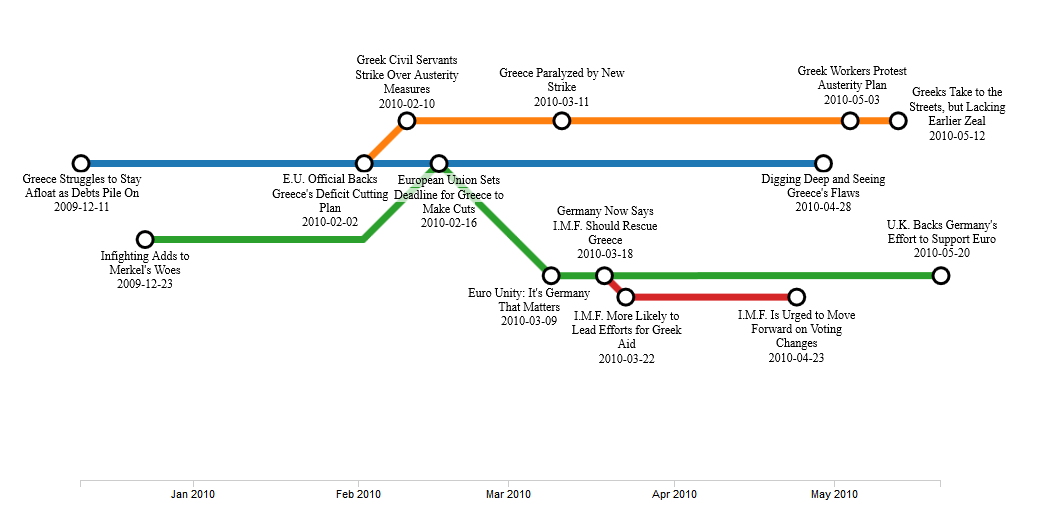
\includegraphics[width=\columnwidth]{TimeScaledMap.png}
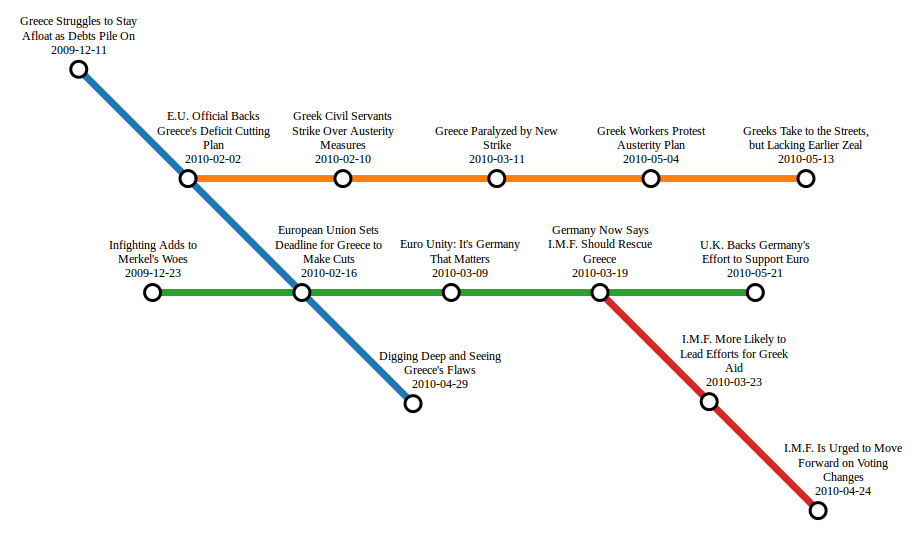
\includegraphics[width=\columnwidth]{TopologicalMap.png}
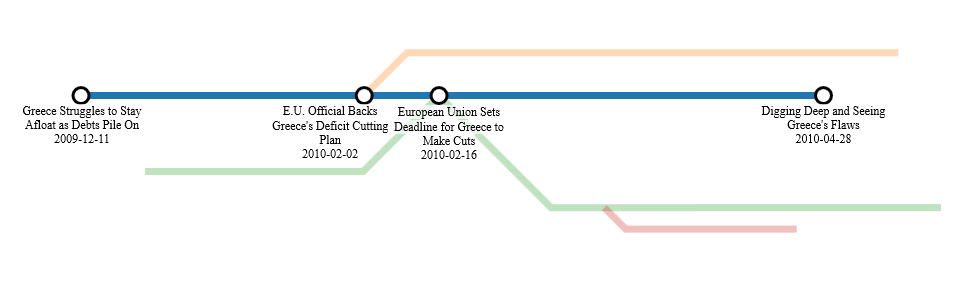
\includegraphics[width=\columnwidth]{Metro1.png}
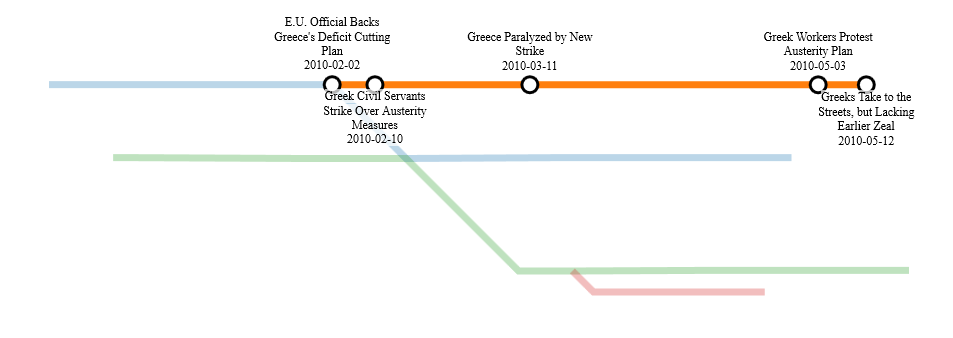
\includegraphics[width=\columnwidth]{Metro2.png}
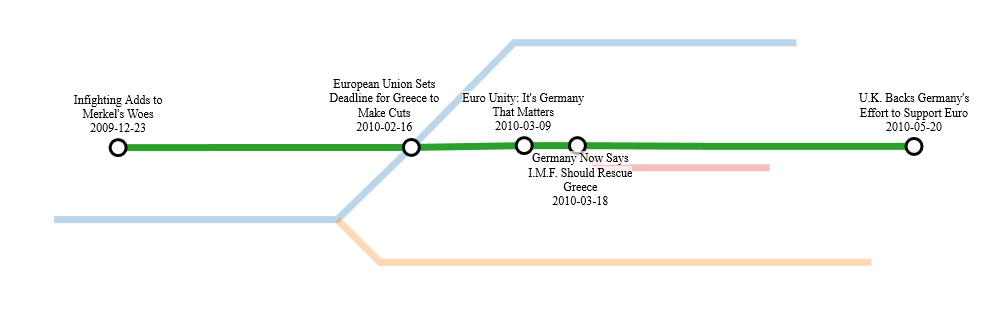
\includegraphics[width=\columnwidth]{Metro3.png}
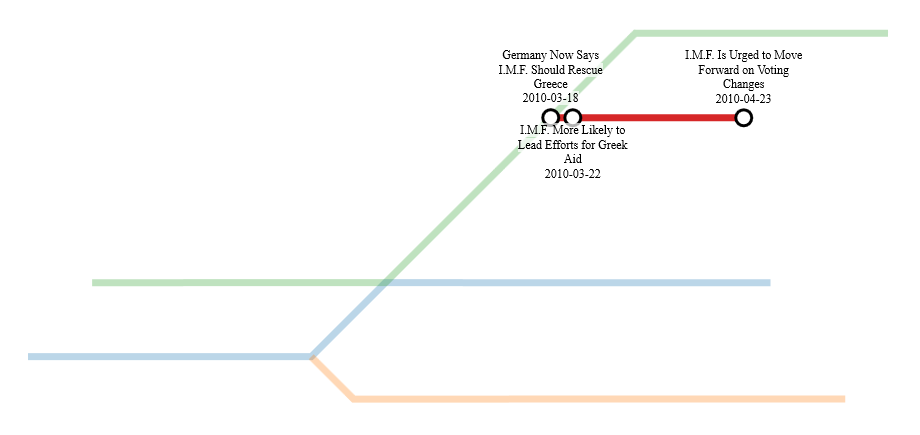
\includegraphics[width=\columnwidth]{Metro4.png}

One of the issues that arose as we implemented the forces was the confounding effect some would have on each other.  As the number of forces increased, the complexity of some of the interactions would push the nodes into unintended locations.  The cooling factor helped mitigate some of the issues by parameterizing how strong different forces were at different times, but there were still some that interfered with each other detrimentally.  For example, in the Greek map we had two news articles really close together in time, so the timeforce tried to push them together (but only along the x-axis).  On the other hand, the octoforce determined that the node was close to vertical, so it tried to push the nodes to vertical, and combined the node would fly off the page.  However, by carefully controlling the force strengths, and locking nodes when necessary, we were able to create all the maps in our demonstrations on the order of five minutes.  

\section{Discussion}

During the process of adding our own forces to the force-directed graph model, we gained a few insights from how to better integrate many different potentially conflicting forces in the same simulation.  We discovered that just a straightforward application of our forces would not lead to intuitive behavior from the model.  If we just applied our forces strongly from the start, we would end up with very messy map states.  For example, when octoforce is enforced strongly from the start, we will end up with many nodes overlapping since the octoforce encourages many parallel lines, and they often end up on top of each other.  

By adopting d3’s annealing model, we had a more natural way to integrate the original forces with our new forces.  In our first iteration attempt to integrate the forces smoothly, the original charge and gravity layout forces were stronger when the model first heats up, and then they gradually weakened as the octoforce and timeforce overtook it when the model cooled down.  This helped the overlapping problem because the node charges did a good job to prevent that, and then our forces help align the map to a final cleaner state.  

However, this also caused the nodes to keep “bouncing” between the beginning warm state when the original forced-directed graph’s forces were dominant and the ending cooled state when the timeforce was dominant.  When the timeforce was relaxed at the beginning of annealing, the nodes would snap back to a ball like a simple force-directed layout, and then they would slowly stretch out to the time-scaled locations.  This was very disorienting and made the map hard to edit because it was always unstable.  
    It turns out that we had to treat our forces differently with different priorities.  To get a more intuitive behavior, we had to enforce timeforce strongly at all times, while the annealing schedule only affected all the other forces.  This finally gave us a more intuitive behavior for the map editor that allowed for pretty quick creation of maps.  

We learned a lot about how to debug and tune force directed layouts. We think that the “debug panel” for our force layout, which we’ve initialized to generically useful settings and which can very simply be adjusted further by a user, is something that anyone who is making a force directed layout could use (and we are looking to factor it out into a reusable bit of code to help others building a force layout.)

On the viewer side, we found that most of our decisions were quite effective. our project seeks to provide an accessible viewer for metro maps, a new way of looking at complex stories which cannot be summarized on a simple timeline. The hope of the demo is to introduce the audience to the concept of a metro map, and how to interpret it.  In order to facilitate faster comprehension of the metromap, we added the feature to focus on specific news thread and dim the rest, as well as node highlighting when viewing the full text of a news article and a short tutorial.   The slideshow we introduce to walk through functionality served successfully as a tutorial. Users during informal testing and at the poster session demos found the layout aesthetically pleasing, liked the transitions between line focuses and time constraints, and found node and edge highlighting both to be clear.

Regarding the metro maps concept in general, most demo users saw the aesthetic appeal but not all found it convincingly superior to, say, a simple color-coded timeline in conveying information. A more formal user study with a wider variety of document sets could replicate the superior performance on information summarization that Shahaf’s original research demonstrated \cite{}.

\section{Future Work}

Additional features implemented in future work should be focused on making editing more natural and flexible for those without technical backgrounds. Currently, a great deal of the content must be hard-coded, including xml files supplied by the user with most content. While this is still short of the difficulties that making (even static versions of) these timelines in a presentation or image editing program, it's still not as friendly as letting the user drag-and-drop from query results on a fully pre-processed repository of new stories, with the option to add their own. This would fit with a user-friendly node insertion and path drawing mechanism for our long-term goal, being able to make a metro map from scratch with your own document set (and an easy way to import it); this would let people make metro maps in a wide array of domains (for example, legal decisions, scientific literature, or in-depth analysis of single books).

When multiple constraints are being enforced, our interface should do even more to guide the user through the best practices we’ve learned and described in this work, for instance taking care of the staged enforcement schedules of different constraints that we discuss above.
       Good-looking dynamic focus still requires a fair amount of manual user intervention. A one-click method to focus the map on a single straightened metro line would be useful. Each focused will still have to be manually laid out, but this should be as simple and fast as possible given an initial layout for the full view.
       More complex metro maps, with cycles or with multiple lines crossing a single edge, still present visualization problems. Force-layout can have a difficult time coping with the former, especially when enforcing left-to-right date ordering, while the latter was aesthetically unappealing under schemes we considered.
       More speculative features include a friendlier interface for sharing metro maps, maybe somewhat like manyeyes. Also, a strong alternative to force-based layouts, though it would require significant re-implementation, are mixed-integer programming methods.  

\section{Acknowledgements}

We'd like to acknowledge Dafna Shahaf, for inspiring the project and for many useful discussions, Jeff Heer for teaching the class and important suggestions for features, and Stanford University for making this project possible.

\bibliographystyle{abbrv}
\bibliography{MetroMaps}

\end{document}
